\documentclass{beamer}

\usepackage{kotex}
\usepackage{graphicx,psfrag,amsfonts,amsmath,amssymb}
\usepackage{multicol}
\usepackage{algorithm2e}

\usetheme{metropolis}
\usefonttheme[onlymath]{serif}	% 수식 설정!!
\setbeamertemplate{section in toc}[sections numbered]

\title{Principal Component Models for Sparse Functional Data}
%\date{\today}
\date[Short Occasion]{August 9, 2019}
\author{Hyunsung Kim}
\institute{Department of Statistics\\ Chung-Ang University}

% A subtitle is optional and this may be deleted
\subtitle{}

%\author{F.~Author\inst{1} \and S.~Another\inst{2}}
% - Give the names in the same order as the appear in the paper.
% - Use the \inst{?} command only if the authors have different
%   affiliation.

%\institute[Universities of Somewhere and Elsewhere] % (optional, but mostly needed)
%{
%  \inst{1}%
%  Department of Computer Science\\
%  University of Somewhere
%  \and
%  \inst{2}%
%  Department of Theoretical Philosophy\\
%  University of Elsewhere}
% - Use the \inst command only if there are several affiliations.
% - Keep it simple, no one is interested in your street address.

%\date{Conference Name, 2013}
% - Either use conference name or its abbreviation.
% - Not really informative to the audience, more for people (including
%   yourself) who are reading the slides online

\subject{Functional Data Analysis}
% This is only inserted into the PDF information catalog. Can be left
% out. 

% If you have a file called "university-logo-filename.xxx", where xxx
% is a graphic format that can be processed by latex or pdflatex,
% resp., then you can add a logo as follows:

% \pgfdeclareimage[height=0.5cm]{university-logo}{university-logo-filename}
% \logo{\pgfuseimage{university-logo}}

% Delete this, if you do not want the table of contents to pop up at
% the beginning of each subsection:
\AtBeginSubsection[]
{
  \begin{frame}<beamer>{Outline}
    \tableofcontents[currentsection,currentsubsection]
  \end{frame}
}

\def \bY {\mathbf{Y}}
\def \by {\mathbf{y}}
\def \bX {\mathbf{X}}
\def \bB {\mathbf{B}}
\def \bD {\mathbf{D}}
\def \bbeta {\boldsymbol{\beta}}
\def \btheta {\boldsymbol{\theta}}
\def \bTheta {\boldsymbol{\Theta}}
\def \bepsilon {\boldsymbol{\epsilon}}
\def \balpha {\boldsymbol{\alpha}}
\def \bgamma {\boldsymbol{\gamma}}
\def \bGamma {\boldsymbol{\Gamma}}
\def \bR {\boldsymbol{R}}
\def \bZ {\boldsymbol{Z}}
\def \bG {\boldsymbol{G}}
\def \bu {\boldsymbol{u}}
\def \bV {\boldsymbol{V}}


% Let's get started
\begin{document}

\begin{frame}
  \titlepage
\end{frame}

\begin{frame}{Outline}
  \tableofcontents
  % You might wish to add the option [pausesections]
\end{frame}

% Section and subsections will appear in the presentation overview
% and table of contents.
\section{Reduced rank model}
\begin{frame}{Reduced rank model}
	\begin{block}{Reduced rank model}
	\vspace{0.1cm}
	$$ \bY_i=\mathbf{B}_i\btheta_{\mu}+\mathbf{B}_i\bTheta\balpha_i + \bepsilon_i $$
	where $\btheta_{\mu}$ is $q \times 1$ vector, $\bTheta$ is $ q \times k$ matrix, $\balpha_i$ is $k \times 1$ vector,
	$$ \bepsilon_i \sim (\mathbf{0}, \sigma^2 \mathbf{I}), \ \balpha_i \sim (\mathbf{0}, \mathbf{D}) $$
	subject to
	$$ \bTheta^T \bTheta=\mathbf{I}, \ \int \mathbf{b}(t)^T\mathbf{b}(t)dt=1, \ \int\int \mathbf{b}(t)^T\mathbf{b}(s)dt=0 $$
	\end{block}
	
\end{frame}

\begin{frame}{Reduced rank model}
	\begin{block}{How to find functional PCs}
		\vspace{0.1cm}
		\begin{itemize}
			\item {
				mean function\\
				$\mu(t)=\mathbf{b}(t)^T\btheta_{\mu}$
			}
			\item {
				PC function\\
				$f(t)^T=\mathbf{b}(t)^T\bTheta$
			}
		\end{itemize}
		where $\mathbf{b}(t)$ is the orthonormal spline basis and it can be computed by Gram–Schmidt orthonormalization.(Zhou et al.(2008))
	\end{block}
	
	To find the PC curves, We should estimate $\btheta_{\mu}, \bTheta$.
\end{frame}


\section{EM Algorithm}
\begin{frame}{EM Algorithm}
	\begin{block}{Maximum likelihood (or Penalized least squares)}
		\vspace{0.5cm}
		In the reduced rank model, we should minimized $L(\btheta_{\mu}, \bTheta, \mathbf{D}, \sigma^2)$,
		$$
		\sum_{i=1}^N \bigg \{ (\bY_i-\mathbf{B}_i\btheta_{\mu}-\mathbf{B}_i\bTheta\balpha_i)^T(\bY_i-\mathbf{B}_i\btheta_{\mu}-\mathbf{B}_i\bTheta\balpha_i) + \sigma^2 \balpha_i^T \bD^{-1}\balpha_i \bigg \}
		$$
	\end{block}
	We can minimize this equation using the \texttt{EM} algorithm.
\end{frame}

\begin{frame}{EM Algorithm}
	\begin{block}{Complete data}
		\vspace{0.2cm}
		Let $\balpha_i$ is the latent variable(unobserved), then we can define the complete data $ \mathbf{Z} = (\bY, \balpha)$ and employ the \texttt{EM} algorithm.
	\end{block}
	\vspace{1cm}
	Let $\mathbf\Omega = (\btheta_{\mu}, \bTheta)$ and $L(\mathbf\Omega|\mathbf{Z}) = -L(\btheta_{\mu}, \bTheta, \mathbf{D}, \sigma^2)$, then the minimization problem will be equivalent to maximize $L(\mathbf\Omega|\mathbf{Z})$.
\end{frame}

\begin{frame}{EM Algorithm}
	\begin{block}{E-step}
		\vspace{0.1cm}
		Compute the expectation of the objective function($L(\mathbf\Omega|\mathbf{Z})$) for complete data $\mathbf{Z}$,
		$$
		Q(\mathbf\Omega|\mathbf\Omega^{(t)}) = E\left\{ L(\mathbf\Omega|\mathbf{Z})|\bY,\mathbf\Omega^{(t)} \right\}
		$$
		where $\mathbf\Omega^{(t)} = (\btheta_{\mu}^{(t)}, \bTheta^{(t)})$.\\
		Also we can predict $\balpha_i$ on the E-step.
	\end{block}
\end{frame}

\begin{frame}{EM Algorithm}
	\begin{block}{M-step}
		\vspace{0.1cm}
		$$
		\mathbf\Omega^{(t+1)} = \arg\max_\mathbf\Omega Q(\mathbf\Omega|\mathbf\Omega^{(t)})
		$$
		Also we can estimate $\mathbf{D}, \sigma^2$ on the M-step.
	\end{block}
	\vspace{0.5cm}
	With many \texttt{EM} iterations, it is known to converge to true parameters.
\end{frame}

\begin{frame}{EM Algorithm}
	\begin{algorithm}[H]
		\KwResult{ The procedure to fit the reduced rank model }
		initialization $( \widehat\btheta^{(1)}_\mu, \widehat\bTheta^{(1)}, \widehat{\balpha}^{(1)}_i, \widehat\bD^{(1)}, \widehat{\sigma^2}^{(1)} )$\;
		\For{$i=2$ to $iterations$}
		 {\vspace{0.2cm}
		 	$$
		 	\begin{aligned}
		 		\text{(M-step)}\\
		 		\widehat{\sigma^2}^{(t+1)} \ &\leftarrow \ ( \widehat\btheta^{(t)}_\mu, \widehat\bTheta^{(t)}, \widehat{\balpha}^{(t)}_i, \widehat\bD^{(t)}, \widehat{\sigma^2}^{(t)} )\\
		 		\widehat\bD^{(t+1)}_{jj} \ &\leftarrow \ ( \widehat\bTheta^{(t)}, \widehat{\balpha}^{(t)}_i, \widehat\bD^{(t)}, \widehat{\sigma^2}^{(t+1)} )\\
		 		\widehat\btheta^{(t+1)}_{\mu} \ &\leftarrow \ ( \widehat\bTheta^{(t)}, \widehat{\balpha}^{(t)}_i )\\
		 		\widehat\bTheta^{(t+1)} \ &\leftarrow \ ( \widehat\btheta^{(t)}_\mu, \widehat\bTheta^{(t)}, \widehat{\balpha}^{(t)}_i, \widehat\bD^{(t+1)}, \widehat{\sigma^2}^{(t+1)} )\\
		 		\text{(E-step)}\\
		 		\widehat\balpha_i^{(t+1)} \ &\leftarrow \ ( \widehat\bTheta^{(t+1)}, \widehat{\balpha}^{(t+1)}_i, \widehat\bD^{(t+1)}, \widehat{\sigma^2}^{(t+1)} )
		 	\end{aligned}
		 	$$
	 	 }
	\end{algorithm}
\end{frame}



\section{Applications}
\begin{frame}{Applications}
	\begin{block}{Bone Mineral Density data}
		\begin{itemize}
			\item {
				48 white females			
			}
			\item {
				160 observations
			}
			\item {
				It was measured at the different time points and sparsely observed.
			}
		\end{itemize}
	\end{block}
\end{frame}

\begin{frame}{Applications}
	\begin{figure}[h] %%% t: top, b: bottom, h: here
		\begin{center}
			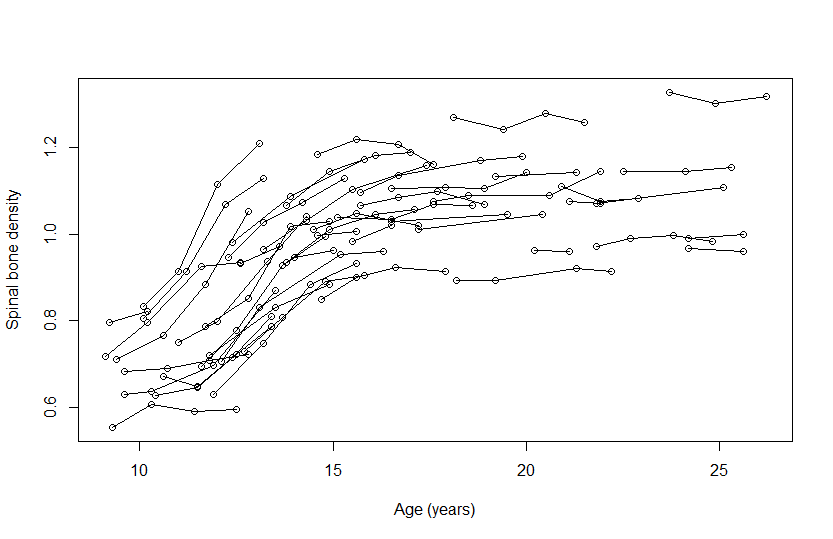
\includegraphics[width=0.8\linewidth]{img/curve.png}
		\end{center}
		\caption{The bone mineral density of 48 females}
		\label{fig:long}
		\label{fig:onecol}
	\end{figure}
	%\end{block}
\end{frame}

\begin{frame}{Applications}
	\begin{itemize}
		\item {
			Fit the reduced rank model using \texttt{EM} algorithm
		}			
		\item {
			Initial values $=0.1 \ (\btheta_{\mu}, \bTheta, \mathbf{D}, \sigma^2, \balpha_i)$
		}
		\item {
			The number of PCs $=2$
		}
		\item {
			$100$ \texttt{EM} iterations
		}
	\end{itemize}
\end{frame}

\begin{frame}{Applications}
	\begin{block}{4 knots}
		\begin{figure}[h] %%% t: top, b: bottom, h: here
			\begin{center}
				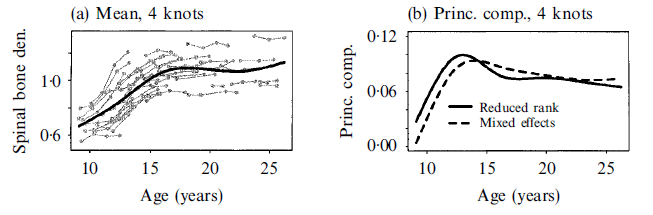
\includegraphics[width=0.8\linewidth]{img/4knots_true.png}
				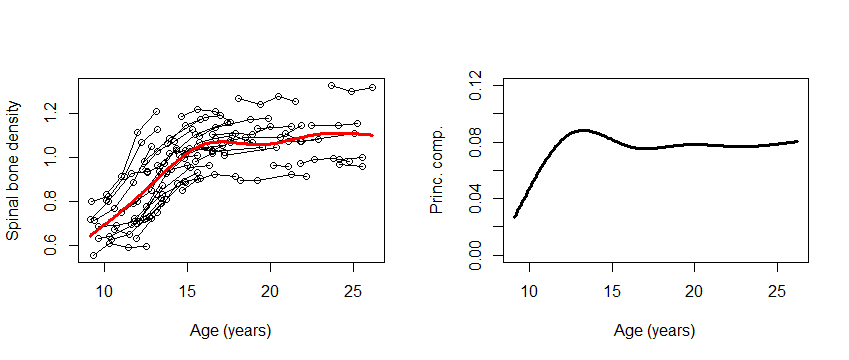
\includegraphics[width=0.8\linewidth]{img/4knots.png}
			\end{center}
			\label{fig:long}
			\label{fig:onecol}
		\end{figure}
	\end{block}
\end{frame}

\begin{frame}{Applications}
	\begin{block}{9 knots}
		\begin{figure}[h] %%% t: top, b: bottom, h: here
			\begin{center}
				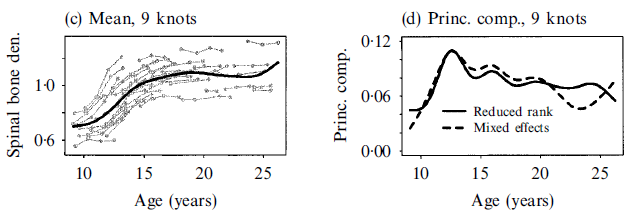
\includegraphics[width=0.8\linewidth]{img/9knots_true.png}
				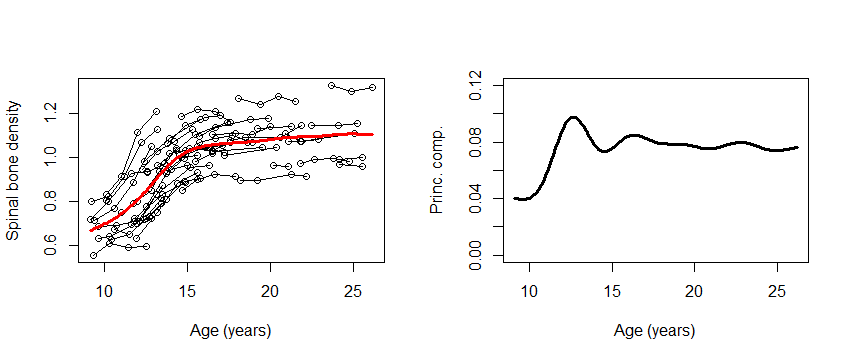
\includegraphics[width=0.8\linewidth]{img/9knots.png}
			\end{center}
			\label{fig:long}
			\label{fig:onecol}
		\end{figure}
	\end{block}
\end{frame}

\begin{frame}{Applications}
	\begin{block}{14 knots}
		\begin{figure}[h] %%% t: top, b: bottom, h: here
			\begin{center}
				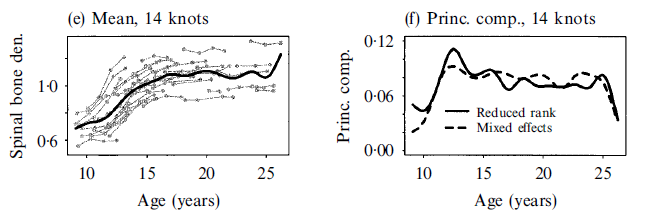
\includegraphics[width=0.8\linewidth]{img/14knots_true.png}
				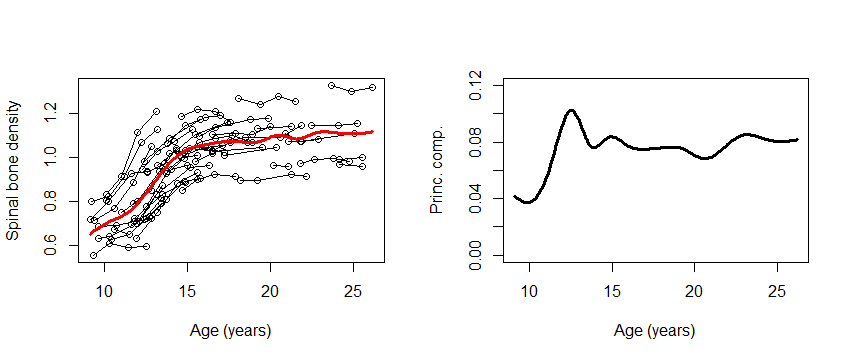
\includegraphics[width=0.8\linewidth]{img/14knots.png}
			\end{center}
			\label{fig:long}
			\label{fig:onecol}
		\end{figure}
	\end{block}
\end{frame}

\begin{frame}{Applications}
	\begin{block}{Loglikelihoods for the reduced rank fits}
		\begin{table}[ht]
			\centering
			\begin{tabular}{ccc}
				\hline
				Number \\of knots& Paper & Coding \\ 
				\hline
				$4$ & 389.22 & 263.22 \\ 
				$9$ & 409.81 & 296.23 \\ 
				$14$ & 411.36 & 308.98 \\ 
				\hline
			\end{tabular}
		\end{table}
	\end{block}
\end{frame}


\appendix
\section{Reference}
\begin{frame}
  \frametitle<presentation>{Reference}
    
  \begin{thebibliography}{10}
  	\beamertemplatearticlebibitems
	% Followed by interesting articles. Keep the list short. 
	 \bibitem{Someone2000}
		James G.M., Hastie T.J., Sugar C.A.
		\newblock Principal component models for sparse functional data
		\newblock {\em Biometrika}, 87(3):587--602,
		2000.
    
  \beamertemplatebookbibitems
  % Start with overview books.
	\bibitem{Author1990}
		J.O. Ramsay, B.W. Silverman.
		\newblock {\em Functional Data Analysis 2nd edition}.
		\newblock Springer, 2005.
		
   	\beamertemplatearticlebibitems
		\bibitem{Someone2008}
		 Zhou L., Huang J.Z., Carroll R.J.
		 \newblock Joint modeling of paired sparse functional data using principal components
		 \newblock {\em Biometrika}, 95(3):601--619,
		 2008.
    

  \end{thebibliography}
\end{frame}


% All of the following is optional and typically not needed. 
%\appendix
%\section<presentation>*{\appendixname}
%\subsection<presentation>*{For Further Reading}
%
%\begin{frame}[allowframebreaks]
%  \frametitle<presentation>{For Further Reading}
%    
%  \begin{thebibliography}{10}
%    
%  \beamertemplatebookbibitems
%  % Start with overview books.
%
%  \bibitem{Author1990}
%    A.~Author.
%    \newblock {\em Handbook of Everything}.
%    \newblock Some Press, 1990.
% 
%    
%  \beamertemplatearticlebibitems
%  % Followed by interesting articles. Keep the list short. 
%
%  \bibitem{Someone2000}
%    S.~Someone.
%    \newblock On this and that.
%    \newblock {\em Journal of This and That}, 2(1):50--100,
%    2000.
%  \end{thebibliography}
%\end{frame}

\end{document}


